% ============================================================
%  SANJEEVANI — SYSTEM DESIGN PPT
%  LaTeX Beamer 16:9, pdfLaTeX-compatible
%  Compile: pdflatex main.tex  (or latexmk -pdf main.tex)
% ============================================================
\documentclass[aspectratio=169,t]{beamer}

\usepackage[utf8]{inputenc}
\usepackage[T1]{fontenc}
\usepackage{lmodern}
\usepackage{tikz}
\usetikzlibrary{shapes.geometric,arrows.meta,positioning,fit,
                backgrounds,calc,decorations.pathreplacing}
% pgfplots not required — all diagrams use TikZ directly
\usepackage{booktabs}
\usepackage{array}
\usepackage{colortbl}
\usepackage{xcolor}
\usepackage{microtype}
\usepackage{hyperref}
\usepackage{multicol}

% ── colour palette (shared with pitch deck) ────────────────
\definecolor{NavyBg}    {HTML}{0D1B2A}
\definecolor{NavyMid}   {HTML}{1A2E44}
\definecolor{NavyLight} {HTML}{243B55}
\definecolor{Teal}      {HTML}{0FA3B1}
\definecolor{TealLight} {HTML}{4DC9D5}
\definecolor{Orange}    {HTML}{F07A25}
\definecolor{OrangeLight}{HTML}{F5A965}
\definecolor{TextMain}  {HTML}{E8F4F8}
\definecolor{TextSub}   {HTML}{9BB5C8}
\definecolor{Green}     {HTML}{4CAF50}
\definecolor{Red}       {HTML}{EF5350}
\definecolor{Purple}    {HTML}{9C27B0}
\definecolor{PurpleLight}{HTML}{CE93D8}

% ── Beamer setup (same as pitch deck) ──────────────────────
\usetheme{default}
\usecolortheme{default}
\setbeamercolor{background canvas}    {bg=NavyBg}
\setbeamercolor{normal text}          {fg=TextMain,bg=NavyBg}
\setbeamercolor{frametitle}           {fg=Teal,bg=NavyBg}
\setbeamercolor{framesubtitle}        {fg=TextSub}
\setbeamercolor{itemize item}         {fg=Teal}
\setbeamercolor{itemize subitem}      {fg=TealLight}
\setbeamercolor{block title}          {fg=NavyBg,bg=Teal}
\setbeamercolor{block body}           {fg=TextMain,bg=NavyMid}
\setbeamercolor{alerted text}         {fg=Orange}
\setbeamercolor{footer}               {fg=TextSub}
\setbeamertemplate{navigation symbols}{}
\setbeamertemplate{itemize item}{\small\textbullet}
\setbeamerfont{frametitle}{size=\large,series=\bfseries}
\setbeamerfont{block title}{size=\normalsize,series=\bfseries}

\setbeamertemplate{footline}{%
  \begin{beamercolorbox}[wd=\paperwidth,ht=2.5ex,dp=1ex,
                         leftskip=3mm,rightskip=3mm]{footer}
    \scriptsize\color{TextSub}%
    Sanjeevani — System Design \hfill How the system works \hfill \insertframenumber
  \end{beamercolorbox}}

% ── TikZ styles ────────────────────────────────────────────
\tikzset{
  layer/.style      = {rectangle,rounded corners=5pt,
                       minimum width=#1,minimum height=0.85cm,
                       align=center,inner sep=5pt},
  implbox/.style    = {layer=2.2cm,fill=Teal!20,draw=Teal,
                       line width=0.8pt,text=TextMain,font=\footnotesize},
  propbox/.style    = {layer=2.2cm,fill=Orange!12,draw=Orange,dashed,
                       line width=0.8pt,text=TextMain,font=\footnotesize},
  navybox/.style    = {rectangle,rounded corners=4pt,fill=NavyMid,
                       draw=Teal!40,line width=0.6pt,text=TextMain,
                       inner sep=6pt,align=center},
  tealbox/.style    = {navybox,fill=Teal!20,draw=Teal},
  orangebox/.style  = {navybox,fill=Orange!15,draw=Orange},
  greenbox/.style   = {navybox,fill=Green!15,draw=Green},
  greybox/.style    = {navybox,fill=NavyLight,draw=TextSub!40},
  dashedbox/.style  = {navybox,draw=TextSub,dashed},
  decbox/.style     = {shape=diamond,fill=Orange!20,draw=Orange,
                       font=\tiny,align=center,inner sep=2pt},
  arrow/.style      = {-{Stealth[length=5pt]},Teal,line width=1.2pt},
  arrowW/.style     = {-{Stealth[length=5pt]},TextSub,line width=0.8pt,dashed},
  arrowO/.style     = {-{Stealth[length=5pt]},Orange,line width=1pt},
  arrowG/.style     = {-{Stealth[length=5pt]},Green,line width=1pt},
}

\newcommand{\teal}[1]{\textcolor{Teal}{#1}}
\newcommand{\orange}[1]{\textcolor{Orange}{#1}}
\newcommand{\tsub}[1]{\textcolor{TextSub}{\small #1}}
\newcommand{\impl}{\,\textcolor{Green}{\scriptsize[impl]}}
\newcommand{\prop}{\,\textcolor{Orange}{\scriptsize[proposed]}}

% ===========================================================
\begin{document}

% ── COVER ───────────────────────────────────────────────────
{
\setbeamertemplate{footline}{}
\begin{frame}[plain]
\begin{tikzpicture}[remember picture,overlay]
  \fill[NavyBg] (current page.south west) rectangle (current page.north east);
  % background geometry
  \fill[Teal!6,opacity=0.7]
        ([xshift=13cm,yshift=2cm]current page.west) circle (5cm);
  \foreach \y in {0.5,1.5,2.5,3.5}{
    \draw[NavyLight,opacity=0.6,line width=0.6pt]
          ([xshift=0cm,yshift=\y cm-2cm]current page.west) --
          ([xshift=16cm,yshift=\y cm-2cm]current page.west);
  }
  % title
  \node[anchor=west,text=Teal,font=\fontsize{36}{42}\selectfont\bfseries]
        at ([xshift=0.8cm,yshift=1.4cm]current page.west) {Sanjeevani};
  \node[anchor=west,text=TextMain,font=\fontsize{18}{22}\selectfont]
        at ([xshift=0.8cm,yshift=0.45cm]current page.west) {How the System Works};
  \draw[Teal,line width=1.5pt]
        ([xshift=0.8cm,yshift=0.05cm]current page.west) --
        ([xshift=10.5cm,yshift=0.05cm]current page.west);
  \node[anchor=west,text=TextSub,font=\small\itshape]
        at ([xshift=0.8cm,yshift=-0.5cm]current page.west)
        {From user action to feedback, progress, and personalised practice.};
  % layer preview
  \node[tealbox,inner sep=6pt,font=\scriptsize,
        text width=3.5cm,align=left]
        at ([xshift=13.5cm,yshift=0.6cm]current page.west)
        {\teal{Stack:}\newline
         Android (Kotlin / Compose)\newline
         MediaPipe · CameraX\newline
         Android TTS · STT\newline
         SharedPreferences\newline
         Fully on-device};
\end{tikzpicture}
\end{frame}
}

% ── SLIDE 1: THE SIMPLEST EXPLANATION ──────────────────────
\begin{frame}{The simplest possible explanation}
\framesubtitle{Five blocks, one sentence}
\begin{center}
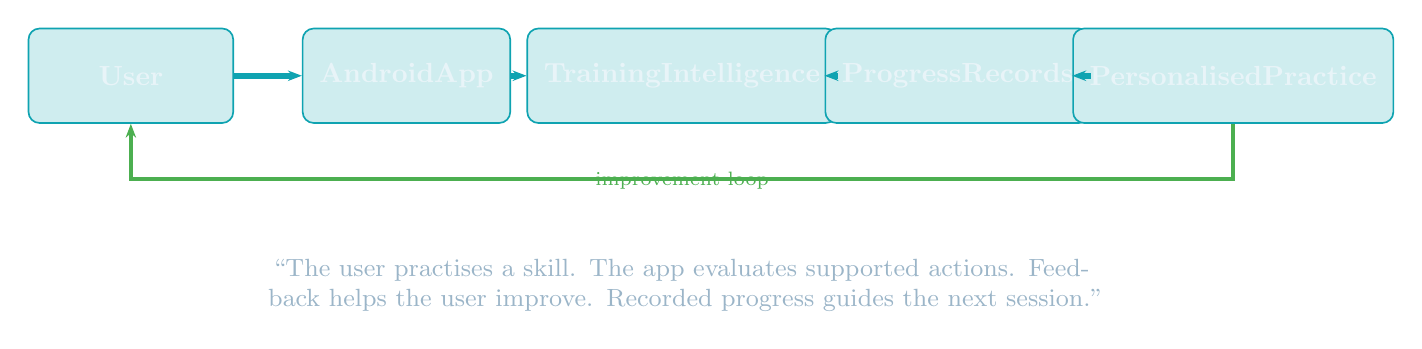
\begin{tikzpicture}[every node/.style={font=\normalsize}]
  \node[tealbox,minimum width=2.6cm,minimum height=1.2cm] (u)
       at (0,0) {\textbf{User}};
  \node[tealbox,minimum width=2.6cm,minimum height=1.2cm] (a)
       at (3.5,0) {\textbf{Android\newline App}};
  \node[tealbox,minimum width=2.6cm,minimum height=1.2cm] (ti)
       at (7.0,0) {\textbf{Training\newline Intelligence}};
  \node[tealbox,minimum width=2.6cm,minimum height=1.2cm] (pr)
       at (10.5,0) {\textbf{Progress\newline Records}};
  \node[tealbox,minimum width=2.6cm,minimum height=1.2cm] (pp)
       at (14.0,0) {\textbf{Personalised\newline Practice}};

  \foreach \a/\b in {u/a, a/ti, ti/pr, pr/pp}
    \draw[arrow,line width=2pt] (\a) -- (\b);

  % return arrow
  \draw[arrowG,line width=1.5pt]
        (pp.south) -- ++(0,-0.7) -| (u.south);
  \node[text=Green,font=\scriptsize,anchor=north] at (7.0,-1.1)
       {improvement loop};

  \node[text=TextSub,font=\small,anchor=north,text width=15cm,align=center]
       at (7.0,-2.2)
       {``The user practises a skill. The app evaluates supported actions. Feedback
         helps the user improve. Recorded progress guides the next session.''};
\end{tikzpicture}
\end{center}
\note{This is the one slide a non-technical judge should be able to read in 10 seconds.
No jargon. Five blocks. One cycle.
Time: ~30 seconds. Transition: "Let me unpack each of those blocks."}
\end{frame}

% ── SLIDE 2: HIGH-LEVEL ARCHITECTURE ─────────────────────
\begin{frame}{High-level architecture}
\framesubtitle{Five layers — \textcolor{Green}{solid = implemented} \quad \textcolor{Orange}{dashed = proposed/not built}}
\begin{center}
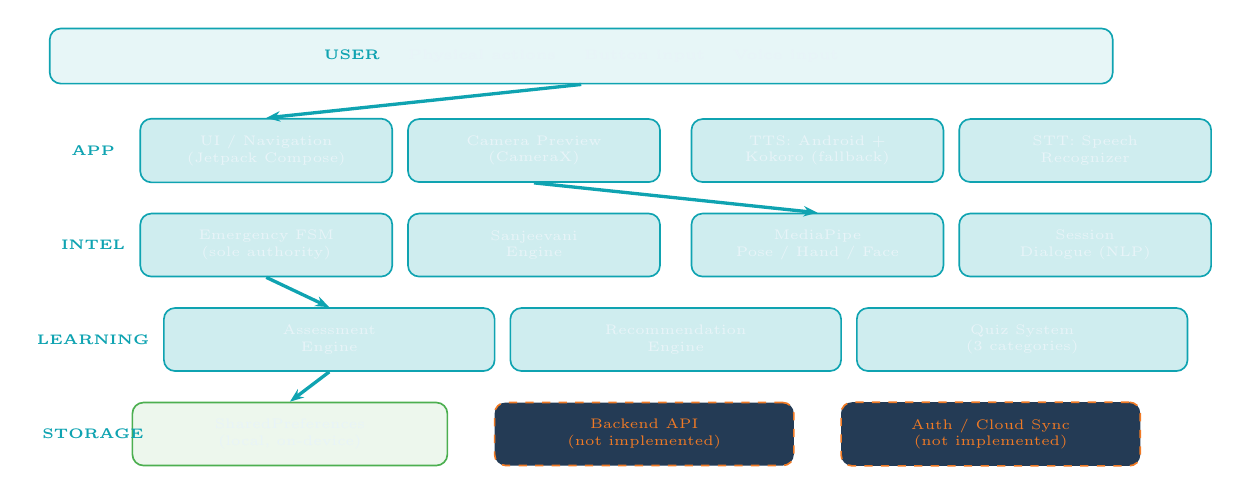
\begin{tikzpicture}[every node/.style={font=\tiny},node distance=0.25cm]
  % ── Row 1: User ──────────────────────────────────────────
  \node[tealbox,minimum width=13.5cm,minimum height=0.7cm,
        fill=Teal!10,draw=Teal,font=\tiny\bfseries]
       (user) at (0,3.2)
       {\teal{USER} \quad Physical actions \quad Button input \quad Voice input};

  % ── Row 2: Android App ───────────────────────────────────
  \node[tealbox,minimum width=3.2cm,minimum height=0.8cm]
       (ui)  at (-4.0,2.0) {UI / Navigation\\ (Jetpack Compose)};
  \node[tealbox,minimum width=3.2cm,minimum height=0.8cm]
       (cam) at (-0.6,2.0) {Camera Preview\\ (CameraX)};
  \node[tealbox,minimum width=3.2cm,minimum height=0.8cm]
       (tts) at (3.0,2.0)  {TTS: Android +\\ Kokoro (fallback)};
  \node[tealbox,minimum width=3.2cm,minimum height=0.8cm]
       (stt) at (6.4,2.0)  {STT: Speech\\ Recognizer};
  \node[text=Teal,font=\tiny\bfseries] at (-6.2,2.0) {APP};

  % ── Row 3: Training Intelligence ─────────────────────────
  \node[tealbox,minimum width=3.2cm,minimum height=0.8cm]
       (fsm) at (-4.0,0.8) {Emergency FSM\\ (sole authority)};
  \node[tealbox,minimum width=3.2cm,minimum height=0.8cm]
       (eng) at (-0.6,0.8) {Sanjeevani\\ Engine};
  \node[tealbox,minimum width=3.2cm,minimum height=0.8cm]
       (mp)  at (3.0,0.8)  {MediaPipe\\ Pose / Hand / Face};
  \node[tealbox,minimum width=3.2cm,minimum height=0.8cm]
       (dlg) at (6.4,0.8)  {Session\\ Dialogue (NLP)};
  \node[text=Teal,font=\tiny\bfseries] at (-6.2,0.8) {INTEL};

  % ── Row 4: Learning ──────────────────────────────────────
  \node[tealbox,minimum width=4.2cm,minimum height=0.8cm]
       (ae)  at (-3.2,-0.4) {Assessment\\ Engine};
  \node[tealbox,minimum width=4.2cm,minimum height=0.8cm]
       (rec) at (1.2,-0.4)  {Recommendation\\ Engine};
  \node[tealbox,minimum width=4.2cm,minimum height=0.8cm]
       (quiz)at (5.6,-0.4)  {Quiz System\\ (3 categories)};
  \node[text=Teal,font=\tiny\bfseries] at (-6.2,-0.4) {LEARNING};

  % ── Row 5: Storage ───────────────────────────────────────
  \node[tealbox,minimum width=4.0cm,minimum height=0.8cm,
        fill=Green!10,draw=Green]
       (sp)  at (-3.7,-1.6) {SharedPreferences\\ (local, on-device)};
  \node[dashedbox,minimum width=3.8cm,minimum height=0.8cm,
        fill=NavyLight,draw=Orange,dashed]
       (api) at (0.8,-1.6)  {\textcolor{Orange}{Backend API}\\ \textcolor{Orange}{(not implemented)}};
  \node[dashedbox,minimum width=3.8cm,minimum height=0.8cm,
        fill=NavyLight,draw=Orange,dashed]
       (auth)at (5.2,-1.6)  {\textcolor{Orange}{Auth / Cloud Sync}\\ \textcolor{Orange}{(not implemented)}};
  \node[text=Teal,font=\tiny\bfseries] at (-6.2,-1.6) {STORAGE};

  % ── Arrows ───────────────────────────────────────────────
  \draw[arrow] (user.south) -- (ui.north);
  \draw[arrow] (cam.south)  -- (mp.north);
  \draw[arrow] (fsm.south)  -- (ae.north);
  \draw[arrow] (ae.south)   -- (sp.north);
\end{tikzpicture}
\end{center}
\note{Walk through top to bottom. Emphasise which dashed boxes are proposed/not yet built (backend, auth, sync, on-device LLM).
The key point: everything that works today is on-device with no network dependency.
Time: ~60 seconds.}
\end{frame}

% ── SLIDE 3: ONE TRAINING SESSION ─────────────────────────
\begin{frame}{What happens during one training session?}
\framesubtitle{Step-by-step flow from module selection to recorded outcome}
\begin{center}
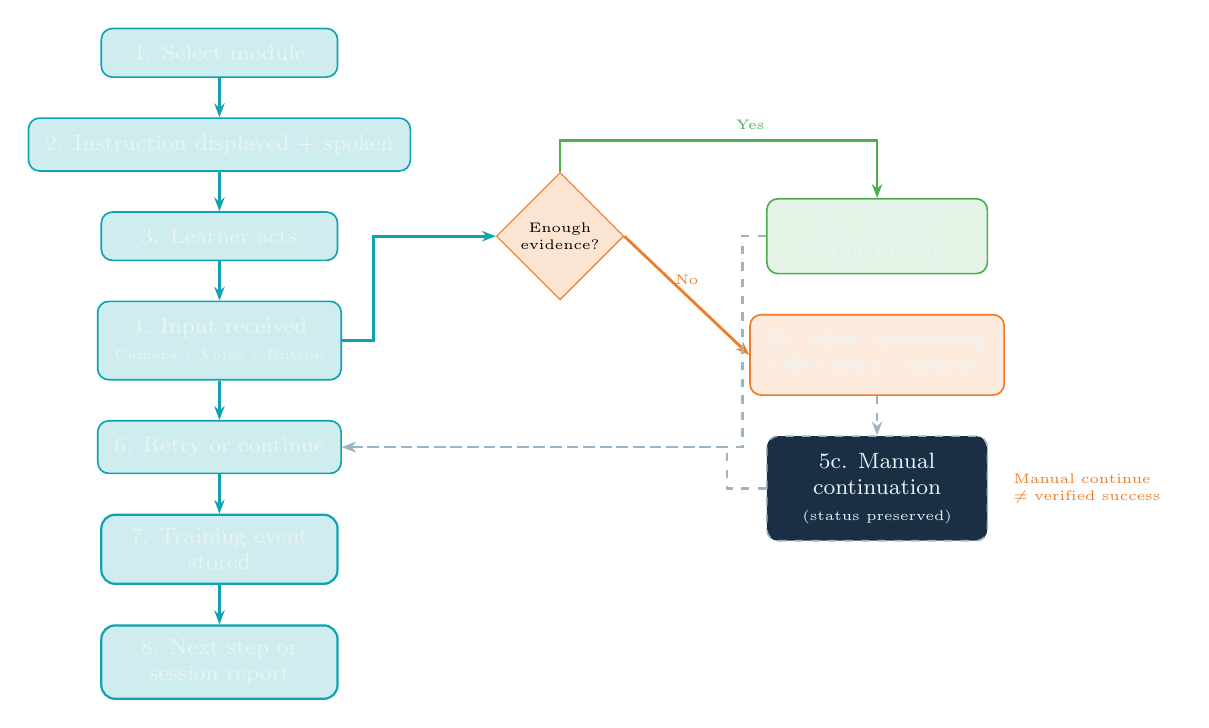
\begin{tikzpicture}[every node/.style={font=\footnotesize},
                    node distance=0.5cm and 1.0cm]

  % flow nodes
  \node[tealbox,minimum width=3.0cm] (sel)   {1. Select module};
  \node[tealbox,minimum width=3.0cm,below=of sel] (inst) {2. Instruction displayed + spoken};
  \node[tealbox,minimum width=3.0cm,below=of inst] (act)  {3. Learner acts};
  \node[tealbox,minimum width=3.0cm,below=of act]  (inp)  {4. Input received\\ {\tiny Camera / Voice / Button}};

  \node[decbox,minimum size=1.5cm,right=2.0cm of act] (dec)
       {Enough\\evidence?};

  \node[greenbox,minimum width=2.8cm,right=1.8cm of dec] (ok)
       {5a. Record\\ verified result};
  \node[orangebox,minimum width=2.8cm,below=0.5cm of ok] (incon)
       {5b. Show uncertainty\\ Offer retry / manual};
  \node[dashedbox,minimum width=2.8cm,below=0.5cm of incon] (man)
       {5c. Manual\\ continuation\\ {\tiny(status preserved)}};

  \node[tealbox,minimum width=3.0cm,below=of inp] (retry) {6. Retry or continue};
  \node[implbox,layer=3.0cm,below=of retry]       (rec)   {7. Training event\\ stored};
  \node[implbox,layer=3.0cm,below=of rec]         (next)  {8. Next step or\\ session report};

  % arrows
  \foreach \a/\b in {sel/inst, inst/act, act/inp, inp/retry, retry/rec, rec/next}
    \draw[arrow] (\a) -- (\b);

  \draw[arrow] (inp.east) -- ++(0.4,0) |- (dec.west);
  \draw[arrowG] (dec.north) -- ++(0,0.4) -| (ok.north)
                node[pos=0.3,above,text=Green,font=\tiny] {Yes};
  \draw[arrowO] (dec.east) -- (incon.west)
                node[midway,above,text=Orange,font=\tiny] {No};
  \draw[arrowW] (incon.south) -- (man.north);
  \draw[arrowW] (man.west)    -- ++(- 0.5,0) |- (retry.east);
  \draw[arrowW] (ok.west)     -- ++(-0.3,0)  |- (retry.east);

  % annotation: manual ≠ verified
  \node[text=Orange,font=\tiny,right=0.2cm of man,anchor=west,text width=2cm]
       {Manual continue\\ $\neq$ verified success};
\end{tikzpicture}
\end{center}
\note{The key architectural decision: the assessment always has an INCONCLUSIVE path.
The app never promotes "I couldn't measure this" to "you got it right."
Manual continuation exists but is stored with its actual status.
Time: ~60 seconds.}
\end{frame}

% ── SLIDE 4: HOW CAMERA FEEDBACK WORKS ────────────────────
\begin{frame}{How camera feedback works}
\framesubtitle{From pixels to supported corrective guidance}
\begin{columns}[T]
\column{0.52\textwidth}
  \begin{center}
  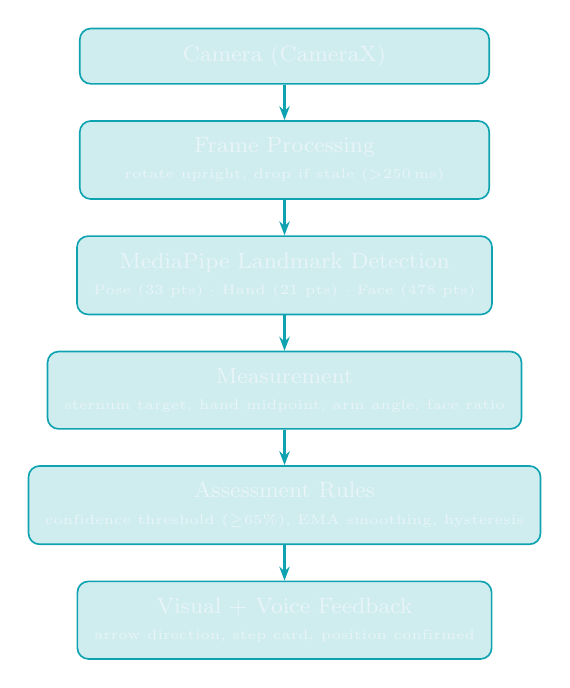
\begin{tikzpicture}[every node/.style={font=\footnotesize},
                      node distance=0.45cm]
    \node[tealbox,minimum width=5.2cm]  (cam)   {Camera (CameraX)};
    \node[tealbox,minimum width=5.2cm,below=of cam]  (fp)
         {Frame Processing\\ {\tiny rotate upright, drop if stale (>250\,ms)}};
    \node[tealbox,minimum width=5.2cm,below=of fp]   (mp)
         {MediaPipe Landmark Detection\\ {\tiny Pose (33 pts) · Hand (21 pts) · Face (478 pts)}};
    \node[tealbox,minimum width=5.2cm,below=of mp]   (meas)
         {Measurement\\ {\tiny sternum target, hand midpoint, arm angle, face ratio}};
    \node[tealbox,minimum width=5.2cm,below=of meas] (asses)
         {Assessment Rules\\ {\tiny confidence threshold ($\geq$65\%), EMA smoothing, hysteresis}};
    \node[tealbox,minimum width=5.2cm,below=of asses] (fb)
         {Visual + Voice Feedback\\ {\tiny arrow direction, step card, position confirmed}};

    \foreach \a/\b in {cam/fp, fp/mp, mp/meas, meas/asses, asses/fb}
      \draw[arrow] (\a) -- (\b);
  \end{tikzpicture}
  \end{center}
\column{0.45\textwidth}
  \vspace{0.5cm}
  \textbf{\teal{Four possible assessment states:}}\smallskip

  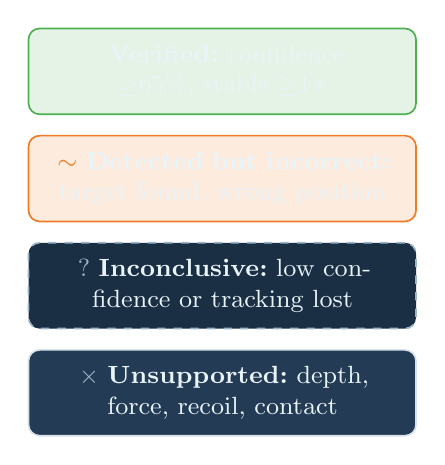
\begin{tikzpicture}[every node/.style={font=\small}]
    \node[greenbox,text width=4.5cm,inner sep=6pt]  (v) at (0,0)
         {\textcolor{Green}{$\checkmark$}\ \textbf{Verified:}\
          confidence $\geq$65\%, stable $\geq$1\,s};
    \node[orangebox,text width=4.5cm,inner sep=6pt,below=0.25cm of v] (inc)
         {\textcolor{Orange}{$\sim$}\ \textbf{Detected but incorrect:}\
          target found, wrong position};
    \node[dashedbox,text width=4.5cm,inner sep=6pt,below=0.25cm of inc] (unc)
         {\textcolor{TextSub}{$?$}\ \textbf{Inconclusive:}\
          low confidence or tracking lost};
    \node[greybox,text width=4.5cm,inner sep=6pt,below=0.25cm of unc] (uns)
         {\textcolor{TextSub}{$\times$}\ \textbf{Unsupported:}\
          depth, force, recoil, contact};
  \end{tikzpicture}

  \vspace{0.4cm}
  \textcolor{TextSub}{\scriptsize
    A detected wrist position does not verify contact or pressure.
    A position landmark does not prove clinical technique.
    Low-confidence frames are discarded, not averaged upward.}
\end{columns}
\note{The camera pipeline is honest: most clinically important quantities (depth, force, delivery) are in the "Unsupported" category.
Explain EMA (exponential moving average) as a smoothing filter that prevents a single good frame from triggering a false positive.
Time: ~60 seconds.}
\end{frame}

% ── SLIDE 5: SHARED ARCHITECTURE, SEPARATE RULES ──────────
\begin{frame}{Shared infrastructure, distinct assessment rules}
\framesubtitle{Three modules — one engine, separate validation logic}
\begin{center}
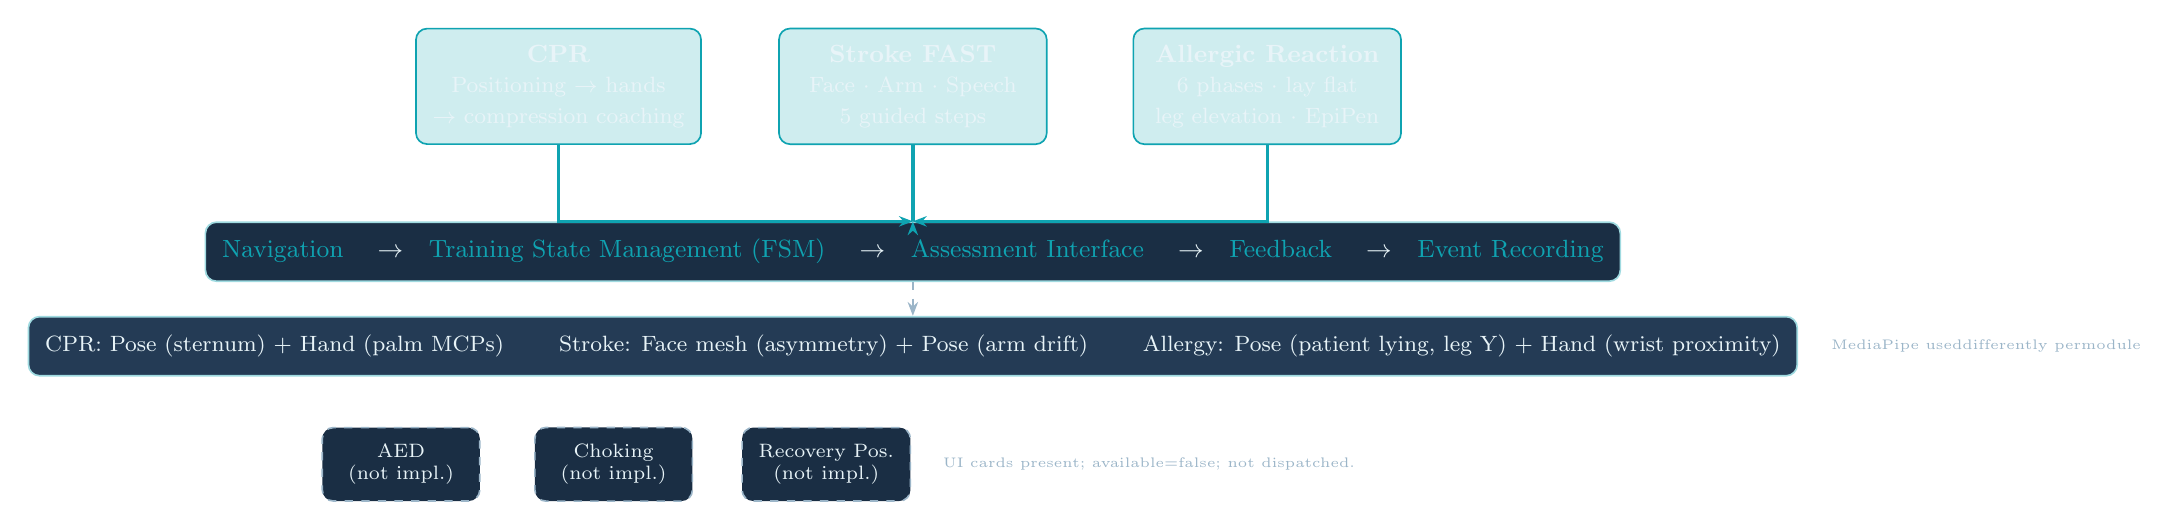
\begin{tikzpicture}[every node/.style={font=\small},
                    node distance=0.5cm and 0.8cm]

  % Three module boxes
  \node[tealbox,minimum width=3.4cm,minimum height=1.4cm] (cpr)
       at (-4.5,0) {\textbf{CPR}\\
                  {\footnotesize Positioning $\rightarrow$ hands}\\
                  {\footnotesize $\rightarrow$ compression coaching}};
  \node[tealbox,minimum width=3.4cm,minimum height=1.4cm] (str)
       at (0,0)    {\textbf{Stroke FAST}\\
                   {\footnotesize Face $\cdot$ Arm $\cdot$ Speech}\\
                   {\footnotesize 5 guided steps}};
  \node[tealbox,minimum width=3.4cm,minimum height=1.4cm] (all)
       at (4.5,0)  {\textbf{Allergic Reaction}\\
                   {\footnotesize 6 phases $\cdot$ lay flat}\\
                   {\footnotesize leg elevation $\cdot$ EpiPen}};

  % shared infrastructure bar
  \node[navybox,fill=NavyMid,draw=Teal!40,minimum width=13.5cm,
        minimum height=0.75cm] (inf) at (0,-2.1)
       {\teal{Navigation} \quad$\rightarrow$\quad
        \teal{Training State Management (FSM)} \quad$\rightarrow$\quad
        \teal{Assessment Interface} \quad$\rightarrow$\quad
        \teal{Feedback} \quad$\rightarrow$\quad
        \teal{Event Recording}};

  % connecting arrows
  \foreach \m in {cpr, str, all}
    \draw[arrow] (\m.south) -- ++(0,-0.5) |- (inf.north);

  % MediaPipe box — used differently per module
  \node[navybox,fill=NavyLight,minimum width=13.5cm,minimum height=0.75cm]
       (mp) at (0,-3.3)
       {\footnotesize
        CPR: Pose (sternum) + Hand (palm MCPs) \qquad
        Stroke: Face mesh (asymmetry) + Pose (arm drift) \qquad
        Allergy: Pose (patient lying, leg Y) + Hand (wrist proximity)};

  \draw[arrowW] (inf.south) -- (mp.north);
  \node[text=TextSub,font=\tiny,right=0.3cm of mp.east,anchor=west]
       {MediaPipe used\\ differently per\\ module};

  % unavailable modules
  \node[dashedbox,minimum width=2.0cm,minimum height=0.9cm,font=\scriptsize]
       (aed) at (-6.5,-4.8) {AED\\ (not impl.)};
  \node[dashedbox,minimum width=2.0cm,minimum height=0.9cm,font=\scriptsize]
       (cho) at (-3.8,-4.8) {Choking\\ (not impl.)};
  \node[dashedbox,minimum width=2.0cm,minimum height=0.9cm,font=\scriptsize]
       (rec) at (-1.1,-4.8) {Recovery Pos.\\ (not impl.)};

  \node[text=TextSub,font=\tiny] at (3.0,-4.8)
       {UI cards present; available=false; not dispatched.};
\end{tikzpicture}
\end{center}
\note{The shared infrastructure (FSM, assessment engine, event store) means adding a new module does not require rebuilding the plumbing.
Each module's camera usage is different — CPR uses hand landmarks very differently from Allergy's wrist-to-thigh proximity test.
The three unavailable modules are visible in the UI as coming-soon cards.
Time: ~50 seconds.}
\end{frame}

% ── SLIDE 6: HOW A MISTAKE BECOMES INSIGHT ────────────────
\begin{frame}{How a mistake becomes a learning insight}
\framesubtitle{The data path from attempt to analytics}
\begin{center}
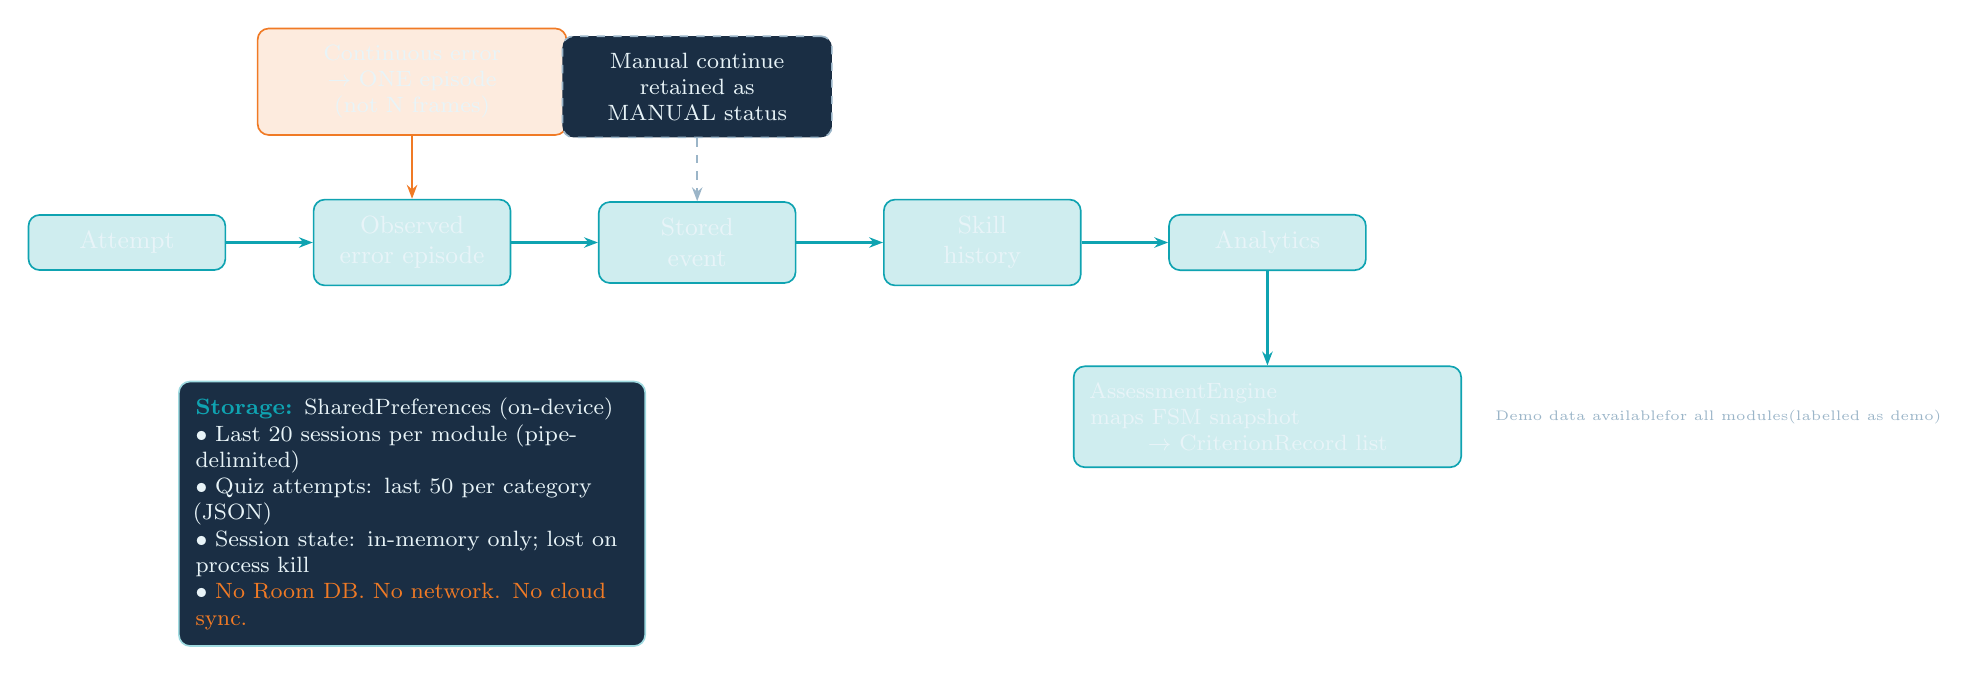
\begin{tikzpicture}[every node/.style={font=\small},
                    node distance=0.5cm and 1.1cm]

  \node[tealbox,minimum width=2.5cm] (att)  {Attempt};
  \node[tealbox,minimum width=2.5cm,right=of att] (obs)
       {Observed\\ error episode};
  \node[tealbox,minimum width=2.5cm,right=of obs] (ev)
       {Stored\\ event};
  \node[tealbox,minimum width=2.5cm,right=of ev]  (hist)
       {Skill\\ history};
  \node[tealbox,minimum width=2.5cm,right=of hist] (anal)
       {Analytics};

  \foreach \a/\b in {att/obs, obs/ev, ev/hist, hist/anal}
    \draw[arrow] (\a) -- (\b);

  % Deduplication note
  \node[orangebox,text width=3.5cm,align=center,font=\footnotesize,
        above=0.8cm of obs] (ded) {Continuous error\\ $\rightarrow$ ONE episode\\ (not N frames)};
  \draw[arrowO] (ded.south) -- (obs.north);

  % Status preservation note
  \node[dashedbox,text width=3.0cm,align=center,font=\footnotesize,
        above=0.8cm of ev] (stat) {Manual continue\\ retained as\\ MANUAL status};
  \draw[arrowW] (stat.south) -- (ev.north);

  % Storage implementation note
  \node[navybox,text width=5.5cm,align=left,font=\footnotesize,
        below=1.2cm of obs] (store) {
    \teal{\textbf{Storage:}} SharedPreferences (on-device)\newline
    $\bullet$\ Last 20 sessions per module (pipe-delimited)\newline
    $\bullet$\ Quiz attempts: last 50 per category (JSON)\newline
    $\bullet$\ Session state: in-memory only; lost on process kill\newline
    $\bullet$\ \orange{No Room DB. No network. No cloud sync.}
  };

  % Assessment engine
  \node[tealbox,text width=4.5cm,align=center,font=\footnotesize,
        below=1.2cm of anal] (ae) {
    AssessmentEngine\newline maps FSM snapshot\newline$\rightarrow$ CriterionRecord list
  };
  \draw[arrow] (anal.south) -- (ae.north);

  % Demo data note
  \node[text=TextSub,font=\tiny,right=0.3cm of ae.east,anchor=west]
       {Demo data available\\ for all modules\\ (labelled as demo)};
\end{tikzpicture}
\end{center}
\note{The deduplication point is critical for credible analytics.
If we counted every 30-ms camera frame as a separate "error event," we would generate thousands of misleading data points from a single 3-second positioning mistake.
One episode = one meaningful observation.
Time: ~55 seconds.}
\end{frame}

% ── SLIDE 7: TARGETED PRACTICE ────────────────────────────
\begin{frame}{How targeted practice works}
\framesubtitle{From skill history to the right exercise — reusing the same mechanism}
\begin{center}
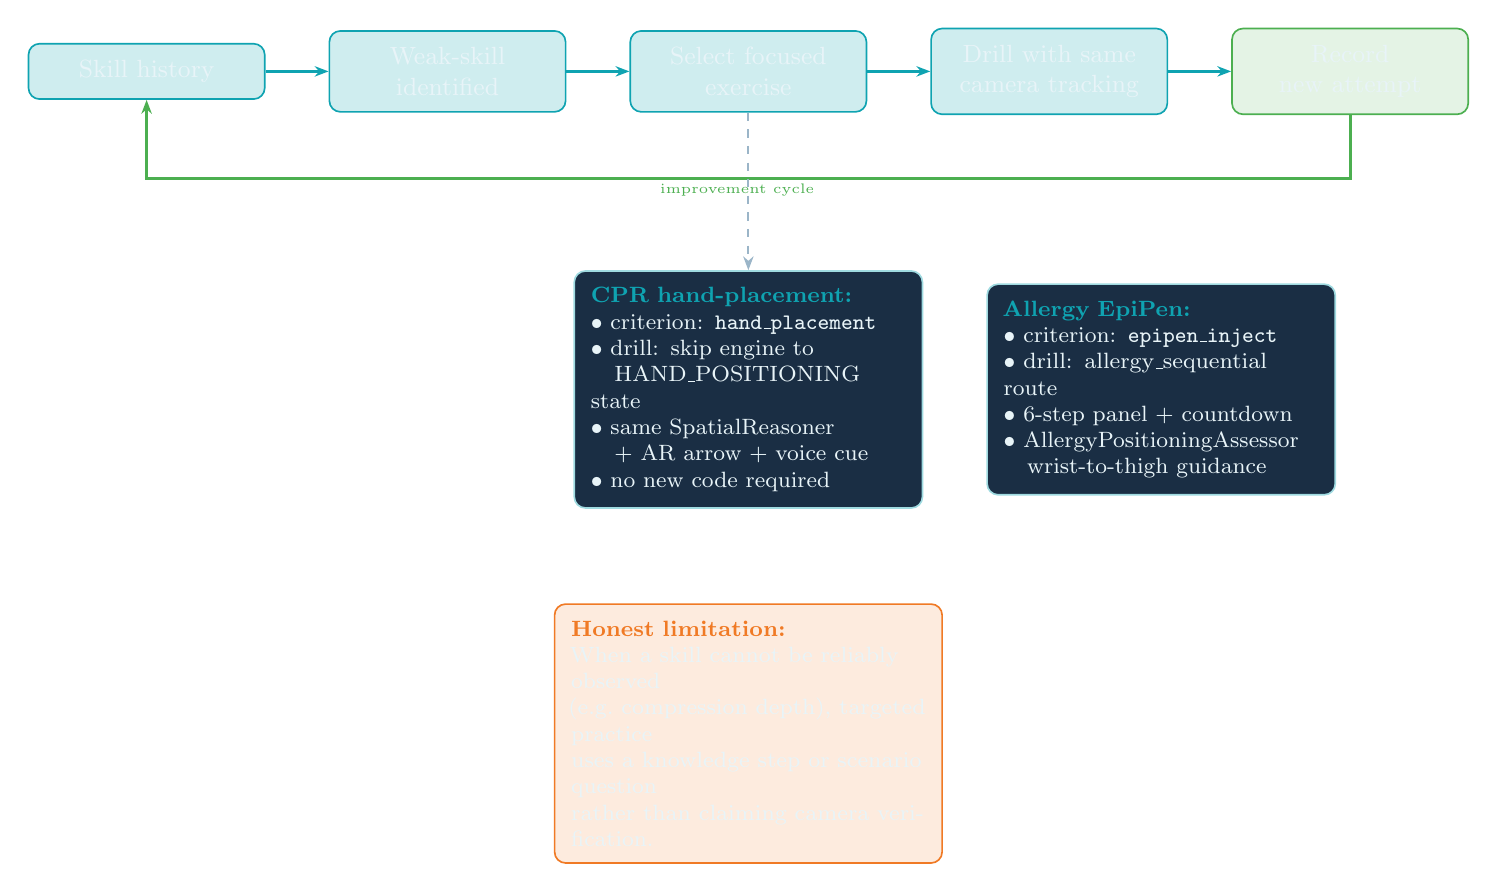
\begin{tikzpicture}[every node/.style={font=\small},
                    node distance=0.55cm and 0.8cm]

  % main path
  \node[tealbox,minimum width=3.0cm] (hist) {Skill history};
  \node[tealbox,minimum width=3.0cm,right=of hist]  (weak)
       {Weak-skill\\ identified};
  \node[tealbox,minimum width=3.0cm,right=of weak]  (sel)
       {Select focused\\ exercise};
  \node[tealbox,minimum width=3.0cm,right=of sel]   (drll)
       {Drill with same\\ camera tracking};
  \node[greenbox,minimum width=3.0cm,right=of drll]  (rec)
       {Record\\ new attempt};

  \foreach \a/\b in {hist/weak, weak/sel, sel/drll, drll/rec}
    \draw[arrow] (\a) -- (\b);

  % improvement cycle back
  \draw[arrowG] (rec.south) -- ++(0,-0.8) -| (hist.south);
  \node[text=Green,font=\tiny,anchor=north] at (7.5,-1.3) {improvement cycle};

  % CPR example callout
  \node[navybox,text width=4.0cm,align=left,font=\footnotesize,
        below=2.0cm of sel] (ex) {
    \teal{\textbf{CPR hand-placement:}}\newline
    $\bullet$\ criterion: \texttt{hand\_placement}\newline
    $\bullet$\ drill: skip engine to\\ \quad HAND\_POSITIONING state\newline
    $\bullet$\ same SpatialReasoner\\ $\quad$+ AR arrow + voice cue\newline
    $\bullet$\ no new code required
  };
  \draw[arrowW] (sel.south) -- (ex.north);

  % Allergy example
  \node[navybox,text width=4.0cm,align=left,font=\footnotesize,
        right=0.8cm of ex] (ex2) {
    \teal{\textbf{Allergy EpiPen:}}\newline
    $\bullet$\ criterion: \texttt{epipen\_inject}\newline
    $\bullet$\ drill: allergy\_sequential route\newline
    $\bullet$\ 6-step panel + countdown\newline
    $\bullet$\ AllergyPositioningAssessor\\ $\quad$wrist-to-thigh guidance
  };

  % Honest limitation box
  \node[orangebox,text width=4.5cm,align=left,font=\footnotesize,
        below=1.2cm of ex] (lim) {
    \orange{\textbf{Honest limitation:}}\newline
    When a skill cannot be reliably observed\newline
    (e.g.\ compression depth), targeted practice\newline
    uses a knowledge step or scenario question\newline
    rather than claiming camera verification.
  };
\end{tikzpicture}
\end{center}
\note{The "reuse the same mechanism" principle means there is no artificial distinction between a drill and a training session — the same engine, the same camera assessment, the same feedback — just entering at the relevant step.
Time: ~55 seconds.}
\end{frame}

% ── SLIDE 8: REDUCING EQUIPMENT DEPENDENCE ────────────────
\begin{frame}{How Sanjeevani can reduce equipment dependence}
\framesubtitle{What a phone can support — and what it cannot replace}
\begin{columns}[T]
\column{0.52\textwidth}
  \begin{center}
  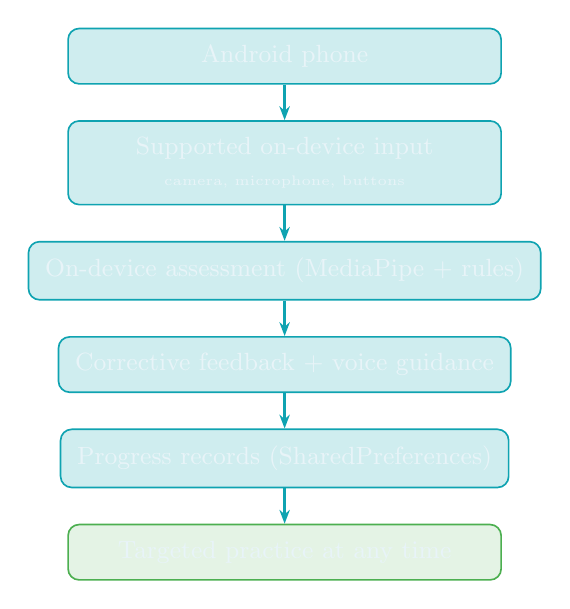
\begin{tikzpicture}[every node/.style={font=\small},
                      node distance=0.45cm]
    \node[tealbox,minimum width=5.5cm] (ph) {Android phone};
    \node[tealbox,minimum width=5.5cm,below=of ph] (si)
         {Supported on-device input\\ {\tiny camera, microphone, buttons}};
    \node[tealbox,minimum width=5.5cm,below=of si] (as)
         {On-device assessment (MediaPipe + rules)};
    \node[tealbox,minimum width=5.5cm,below=of as] (fb)
         {Corrective feedback + voice guidance};
    \node[tealbox,minimum width=5.5cm,below=of fb] (pr)
         {Progress records (SharedPreferences)};
    \node[greenbox,minimum width=5.5cm,below=of pr] (tp)
         {Targeted practice at any time};

    \foreach \a/\b in {ph/si, si/as, as/fb, fb/pr, pr/tp}
      \draw[arrow] (\a) -- (\b);
  \end{tikzpicture}
  \end{center}

\column{0.45\textwidth}
  \vspace{0.5cm}
  \begin{block}{\teal{What this enables}}
    \footnotesize
    $\checkmark$\ Repeat practice sessions without scheduling\newline
    $\checkmark$\ Skill-targeted revision between workshops\newline
    $\checkmark$\ No internet or account required\newline
    $\checkmark$\ Progress persists across sessions on device
  \end{block}
  \vspace{0.3cm}
  \begin{alertblock}{\orange{What it does not replace}}
    \small
    \textbf{Digital feedback is limited to supported, validated observations.
    Physical mannequins and qualified instructors remain important
    wherever hands-on verification or supervised training is required.}\medskip

    \footnotesize
    $\times$\ Compression depth / force / recoil\newline
    $\times$\ Actual medication delivery\newline
    $\times$\ Clinical technique certification\newline
    $\times$\ Emergency dispatch or diagnosis
  \end{alertblock}
\end{columns}
\note{This slide directly addresses the "but isn't a phone a toy compared to a real mannequin?" objection.
Answer: yes, for some things. No, for others. The phone handles repetition, guidance, and awareness. The mannequin handles force and depth feedback.
Both have a place. Sanjeevani reduces the barrier to frequent revision — it does not eliminate the mannequin session.
Time: ~50 seconds.}
\end{frame}

% ── SLIDE 9: DATA, PRIVACY, RELIABILITY ───────────────────
\begin{frame}{Data, privacy, and reliability}
\framesubtitle{How data flows, what is stored, and how edge cases are handled}

\begin{columns}[T]
\column{0.50\textwidth}
  \begin{block}{\teal{Data flow (implemented)}}
    \footnotesize
    \begin{tabular}{@{}ll@{}}
      Camera frames     & On-device only; not stored or transmitted \\
      Voice input       & Android STT; final transcript only \\
      TTS output        & Android TTS + Kokoro; local audio \\
      Training events   & SharedPreferences (local) \\
      Quiz attempts     & SharedPreferences (local) \\
      Network calls     & \orange{None — fully offline} \\
      Raw media stored  & No \\
    \end{tabular}
  \end{block}
  \vspace{0.25cm}
  \begin{block}{\teal{Permissions required}}
    \footnotesize
    \texttt{CAMERA} — CameraX preview + MediaPipe\newline
    \texttt{RECORD\_AUDIO} — Speech recognizer\newline
    No location, contacts, or storage permissions\newline
    Permissions requested at runtime with rationale
  \end{block}

\column{0.47\textwidth}
  \begin{block}{\teal{Edge case handling (implemented)}}
    \footnotesize
    \begin{tabular}{@{}p{2.8cm}p{3.0cm}@{}}
      \textbf{Situation} & \textbf{Behaviour} \\
      \midrule
      Tracking lost      & Rate/cycle invalidated; target frozen \\
      Multi-person frame & Treated as ambiguous; no assessment \\
      Stale camera frame & Dropped ($>$250\,ms age gate) \\
      Stale STT result   & TurnGate (epoch + version) blocks it \\
      App paused         & Active turn cancelled; retry available \\
      Process killed     & In-memory session lost; store data kept \\
      Recognition error  & Retry prompt + tap-button fallback \\
      Duplicate answer   & Version guard prevents double-advance \\
    \end{tabular}
  \end{block}

  \vspace{0.2cm}
  \begin{alertblock}{}
    \footnotesize
    No cloud sync, server backup, or session persistence
    across process death are currently implemented.
    \prop
  \end{alertblock}
\end{columns}
\note{Privacy is a genuine strength: no data leaves the device in the current implementation.
The edge case table shows that the system degrades gracefully — no assessment is promoted to a higher confidence level because tracking was lost.
Time: ~55 seconds.}
\end{frame}

% ── SLIDE 10: THE WHOLE SYSTEM IN ONE PICTURE ─────────────
{
\setbeamertemplate{footline}{}
\begin{frame}[plain]{The entire system in one picture}
\begin{tikzpicture}[remember picture,overlay,every node/.style={font=\small}]
  \fill[NavyBg] (current page.south west) rectangle (current page.north east);

  % circular flow
  \def\cx{8.0}\def\cy{4.3}\def\r{3.5}
  \foreach \i/\lbl/\clr in {
    90/{Learner}/Teal,
    38/{Training Module}/Teal,
    -14/{Observation}/Teal,
    -66/{Assessment}/Teal,
    -118/{Feedback}/Teal,
    -170/{Recorded Progress}/Teal,
    -222/{Targeted Practice}/Teal}{
    \pgfmathsetmacro{\x}{\cx + \r * cos(\i)}
    \pgfmathsetmacro{\y}{\cy + \r * sin(\i)}
    \node[circle,fill=\clr!25,draw=\clr,minimum size=1.5cm,
          align=center,text=TextMain,font=\scriptsize\bfseries]
         at (\x,\y) {\lbl};
  }

  % arcs
  \foreach \s/\e in {90/38, 38/-14, -14/-66, -66/-118, -118/-170, -170/-222}{
    \pgfmathsetmacro{\smid}{(\s+\e)/2}
    \draw[arrow,line width=1.5pt]
          (\cx+\r*cos(\s+10),\cy+\r*sin(\s+10))
       -- (\cx+\r*cos(\e-10),\cy+\r*sin(\e-10));
  }
  % closing arc
  \draw[arrowG,line width=1.5pt]
        (\cx+\r*cos(-222+10),\cy+\r*sin(-222+10))
     -- (\cx+\r*cos(90-10),\cy+\r*sin(90-10));

  % centre text
  \node[circle,fill=NavyMid,draw=Teal!40,minimum size=1.8cm,
        text=Teal,font=\scriptsize\bfseries,align=center]
       at (\cx,\cy) {Sanjeevani};

  % three statements at the bottom
  \node[tealbox,minimum width=4.0cm,font=\small\bfseries]
       at (3.0,0.9) {1. Training is interactive};
  \node[tealbox,minimum width=4.0cm,font=\small\bfseries]
       at (8.0,0.9) {2. Feedback is based on\\ available evidence};
  \node[tealbox,minimum width=4.0cm,font=\small\bfseries]
       at (13.0,0.9) {3. Progress helps identify\\ what to practise next};

  % title
  \node[text=Teal,font=\large\bfseries,anchor=north]
       at (8.0,8.4) {The Sanjeevani loop — from learner to learner};
\end{tikzpicture}
\note{This is the "20-second slide" — a non-technical judge should grasp the entire product concept from this one image.
The three statements at the bottom summarise the engineering principles: interactivity, honest evidence, and data-driven practice.
Total time for system design deck: ~8–10 minutes for full run-through.}
\end{frame}
}

% ── REFERENCES ─────────────────────────────────────────────
\begin{frame}[allowframebreaks]{Technical references}
\footnotesize
\begin{thebibliography}{9}

\bibitem{MediaPipe}
  Google LLC.
  \textit{MediaPipe Solutions — Pose, Hand, and Face Landmarker}.
  Retrieved 2024.
  \url{https://ai.google.dev/edge/mediapipe/solutions/guide}

\bibitem{CameraX}
  Android Developers.
  \textit{CameraX overview}.
  Retrieved 2024.
  \url{https://developer.android.com/media/camera/camerax}

\bibitem{Kokoro}
  k2-fsa / sherpa-onnx.
  \textit{Kokoro TTS — sherpa-onnx Android integration}, v1.13.8.
  \url{https://github.com/k2-fsa/sherpa-onnx}

\bibitem{Compose}
  Android Developers.
  \textit{Jetpack Compose}.
  \url{https://developer.android.com/jetpack/compose}

\bibitem{PoseLandmarks}
  Google LLC.
  \textit{MediaPipe Pose Landmarker landmark indices}.
  \url{https://ai.google.dev/edge/mediapipe/solutions/vision/pose_landmarker}

\bibitem{UKResus}
  Resuscitation Council UK.
  \textit{Adult Basic Life Support Guidelines}, 2021.
  \url{https://www.resus.org.uk/library/2021-resuscitation-guidelines/adult-basic-life-support-guidelines}

\end{thebibliography}
\end{frame}

\end{document}
